%----------------------------------------------------------------------------------------
%	SECTION 7
%----------------------------------------------------------------------------------------

\section{Skills Analysis Conclusion} \label{sec:skills_ccl}


\begin{wrapfigure}[12]{r}{0.25\textwidth}
	\centering
	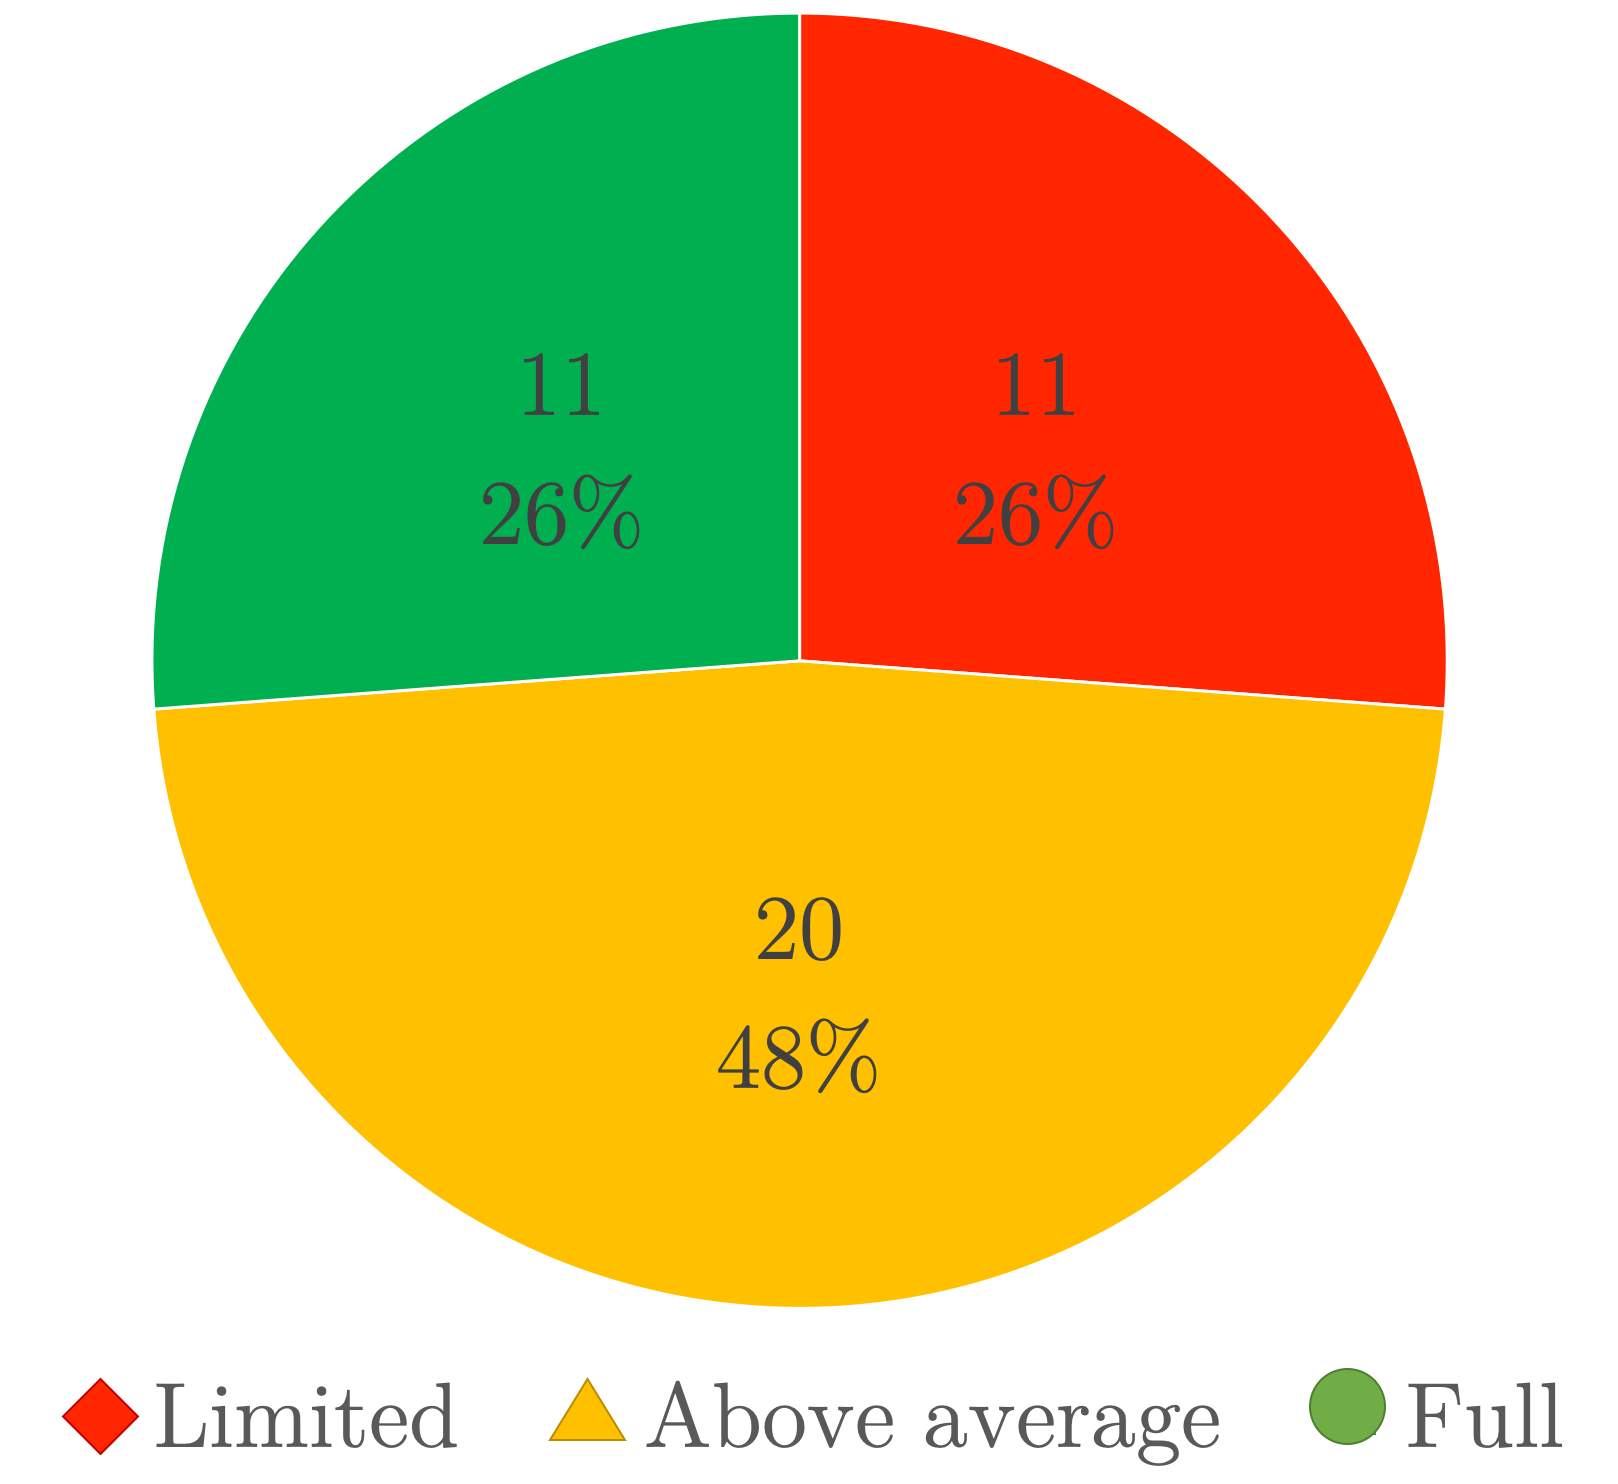
\includegraphics[width=0.25\textwidth]{figures/LO_pie_3.png}
	\rule{0.25\textwidth}{0.5pt} % use line???
	\caption{My achievement of the 42 LOs.}
	\label{fig:LO_pie}
\end{wrapfigure}

Out of the 42 LOs, I have reached full achievement of 11 (26\%), above average achievement of 20 (48\%), and limited achievement of 11 (26\%) (see Figure~\ref{fig:LO_pie}).
Table~\ref{tbl:LOs_summary} summarises my overall achievement levels for all of the LOs.


\begin{table}[htbp]
	\caption{My overall achievement level for every LO.}
	\label{tbl:LOs_summary}
	\centering
	\begin{tabular}{@{}cccc@{}}
		\toprule
		\textbf{} & \littlemaster & \nomaster & \master \\ \midrule
		\multirow{4}{*}{\textbf{SM}} & SM5m & SM1(i, b, m) & SM4m \\
		&  & SM2(i, b, m) &  \\
		&  & SM3(b, m) &  \\
		&  & SM6m &  \\ \midrule
		\multirow{4}{*}{\textbf{EA}} & EA6m & EA1(i, b, m) & EA5m \\
		&  & EA2(i, -) &  \\
		&  & EA3(i, b, m) &  \\
		&  & EA4(i, b, m) &  \\ \midrule
		\multirow{4}{*}{\textbf{D}} & D3(i, b, m) & D4(i, -) & D1(i, -) \\
		&  & D5(i, -) & D2(i, -) \\
		&  & D7m & D6 \\
		&  & D8m &  \\ \midrule
		\multirow{3}{*}{\textbf{EL}} & EL3(i, b, m) & EL1(-, m) & EL4(i, -) \\
		& EL7m & EL2 & EL5(-, m) \\
		&  & EL6(i, b, m) &  \\ \midrule
		\multirow{6}{*}{\textbf{P}} & P4(i, -) & P1(i, -) & P3(i, -) \\
		& P5 & P2(i, b, m) & P7 \\
		& P6(i, -) & P11(i, b, m) &  \\
		& P8 &  &  \\
		& P9m &  &  \\
		& P10(i, b, m) &  &  \\ \midrule
		\multirow{2}{*}{\textbf{G}} &  & G2 & G1 \\
		&  & G3(i, b, m) & G4(i, -) \\ \bottomrule
	\end{tabular}
\end{table}


Interestingly, over the years, my courses and placements have increasingly contributed to my development of the Engineering Council's LOs (see Figure~\ref{fig:cum_courses} in Appendix~\ref{App:matrix}).
In particular, the \LABTitle \space contributed to almost every LO.
The `runners-up' of courses/ placements that have contributed the most to the LOs are \CASTitle, \TPSTitle, \PRJTitle, and Sunamp.
It is surprising that the latter two are runners-up considering my below par performance on the \PRJTitle \space and my very non-technical work experience at Sunamp.






\subsection*{Fully Achieved LOs}

I have fully achieved between one and three LOs from every category.
These have to do with my:
\begin{itemize}
	\item Awareness of and ability to investigate emerging technologies [SM4m, EA5m]
	\item Ability to understand and evaluate user needs [D1(i, -)]
	\item Ability to define and investigate problems [D2(i, -)]
	\item Ability to communicate to technical and non-technical audiences [D6]
	\item Understanding of the need for sustainable development [EL4(i, -)]
	\item Awareness of legal requirements governing engineering activities [EL5(-, m)]
	\item Laboratory skills [P3(i, -)]
	\item Awareness of quality issues and their application to continuous improvement [P7]
	\item Ability to apply additional general skills, e.g. effectively use general IT facilities and exercise personal responsibility in a team [G1, G4(i, -)]
\end{itemize}

Most of the LOs I have fully achieved are related to things I am highly interested in, notably meeting a client's needs, the need for monitoring and evaluation in continuous improvement, and the benefits of developing technologies, all in the interest of sustainable development.




\subsection*{Limited Achievement of LOs}

However, this analysis has highlighted several skills in which I am deficient and need to work harder on to develop.
According to Table~\ref{tbl:LOs_summary}, these have to do with my limited:
\begin{itemize}
	\item Understanding of mathematical and computational models [SM5m]
	\item Ability to work with unfamiliar, uncertain or incomplete information [EA6m, D3(i, b, m), P8]
	\item Knowledge of management techniques [EL3(i, b, m)]
	\item Limited understanding of key drivers for business success [EL7m]
	\item Ability to use technical literature, codes of practice and industry standards [P4(i, -), P6(i, -)]
	\item Knowledge of contractual and legal issues [P5]
	\item Understanding of current practice [P9m]
	\item Ability to apply engineering techniques while considering commercial and industrial constraints [P10m]
\end{itemize}

Additionally, Figure~\ref{fig:cum_LOs} in Appendix~\ref{App:matrix} shows two LO attainment levels that I have no experience in:
\begin{itemize}
	\item EA3m: Ability to apply quantitative and computational methods, using alternative approaches and understanding their limitations, in order to solve engineering problems and implement appropriate action
	\item D4: Apply advanced problem-solving skills, technical knowledge and understanding, to establish rigorous and creative solutions that are fit for purpose for all aspects of the problem including production, operation, maintenance and disposal
\end{itemize}


Table~\ref{tbl:LOs_summary} shows that 55\% of the LOs I have limited achievement in are under the Engineering Practice (P) category.
I believe I should be able to strengthen these skills once I start to work in industry.
Another overarching theme is my difficulty working with uncertain information.
This is most likely linked to my perfectionist and risk-averse tendencies.
To overcome this, I need to practise using my best judgment, making quicker decisions and generally taking more risks.